\section{Results}

In this subsection we first describe the metrics used to evaluate the performance of the models on the skin lesion segmentation task. We then present the experimental environment setup and show the final results.

\subsection{Metrics}

Image segmentation models are mostly evaluated on the basis of how accurately they can predict each pixel. The prediction of the pixels can fall into one of four categories: true positive (TP), true negative (TN) or false positive (FP) and false negative (FN) respectively. The model’s performance is determined by the nature of its prediction and the aforementioned category it belongs to and the computed metrics derived therefrom.

The 2018 lesion segmentation challenge defines the \emph{Threshold Jaccard Index}, averaged over all images in the dataset, as the primary evaluation criteria where the threshold is set to 0.65 \citep{challenge-2018-codella}. The \emph{Jaccard Index}, also called Intersection over Union (IoU), is a method to quantify the percentage of overlap between the target mask (A) and our prediction output (B). It is formally defined as

\begin{equation}
  J(A, B) = \frac{|A \cup B|}{|A \cap B|}
\end{equation}

The Threshold Jaccard Index can then be calculated as

\begin{equation}
  TJ(A, B) = \begin{cases}
      J(A, B), & \text{if}\ J(A, B) \geq{0.65} \\
      0, & \text{otherwise}
    \end{cases}
\end{equation}

The Jaccard Index metric is closely related to the \emph{Dice Coefficient} which is often used as a loss function during training. We use the Dice Coefficient to calculate the area of overlap between the target mask and the predicted mask, defined as

\begin{equation}
  Dice = \frac{2TP}{2TP + FN + FP}
\end{equation}

Furthermore, \emph{accuracy} helps us to track the ratio between correctly predicted pixels over all pixels. For a given prediction, accuracy is defined as

\begin{equation}
  Accuracy = \frac{TP + TN}{TP + FP + TN + FN}
\end{equation}

Finally, \emph{sensitivity} measures the proportion of the correctly identified positives and is   calculated as

\begin{equation}
  Sensitivity = \frac{TP}{TP + FN}
\end{equation}

\emph{Specificity} tells us the proportion of the correctly identified negatives  and can be calculated as

\begin{equation}
  Specificity = \frac{TN}{TN + FP}
\end{equation}


\subsection{Experiments}

\subsubsection{Training Environment Setup}

All experiments were conducted using the same VM setup running Linux 18.04.1-Ubuntu (x86\_64). The underlying hardware contained 54 GiB physical memory, 64-bits Intel(R) Xeon(R) CPU E5-2690 v3 (2.60GHz) and NVIDIA Tesla K80 (8GK210GL, rev a1) GPU with 12 GiB physical memory.

\subsubsection{Approach}

We designed and ran 28 experiments in total. Table \ref{table:experiments} shows an overview of all experiment setups.

\begin{table*}[ht]
  \centering
  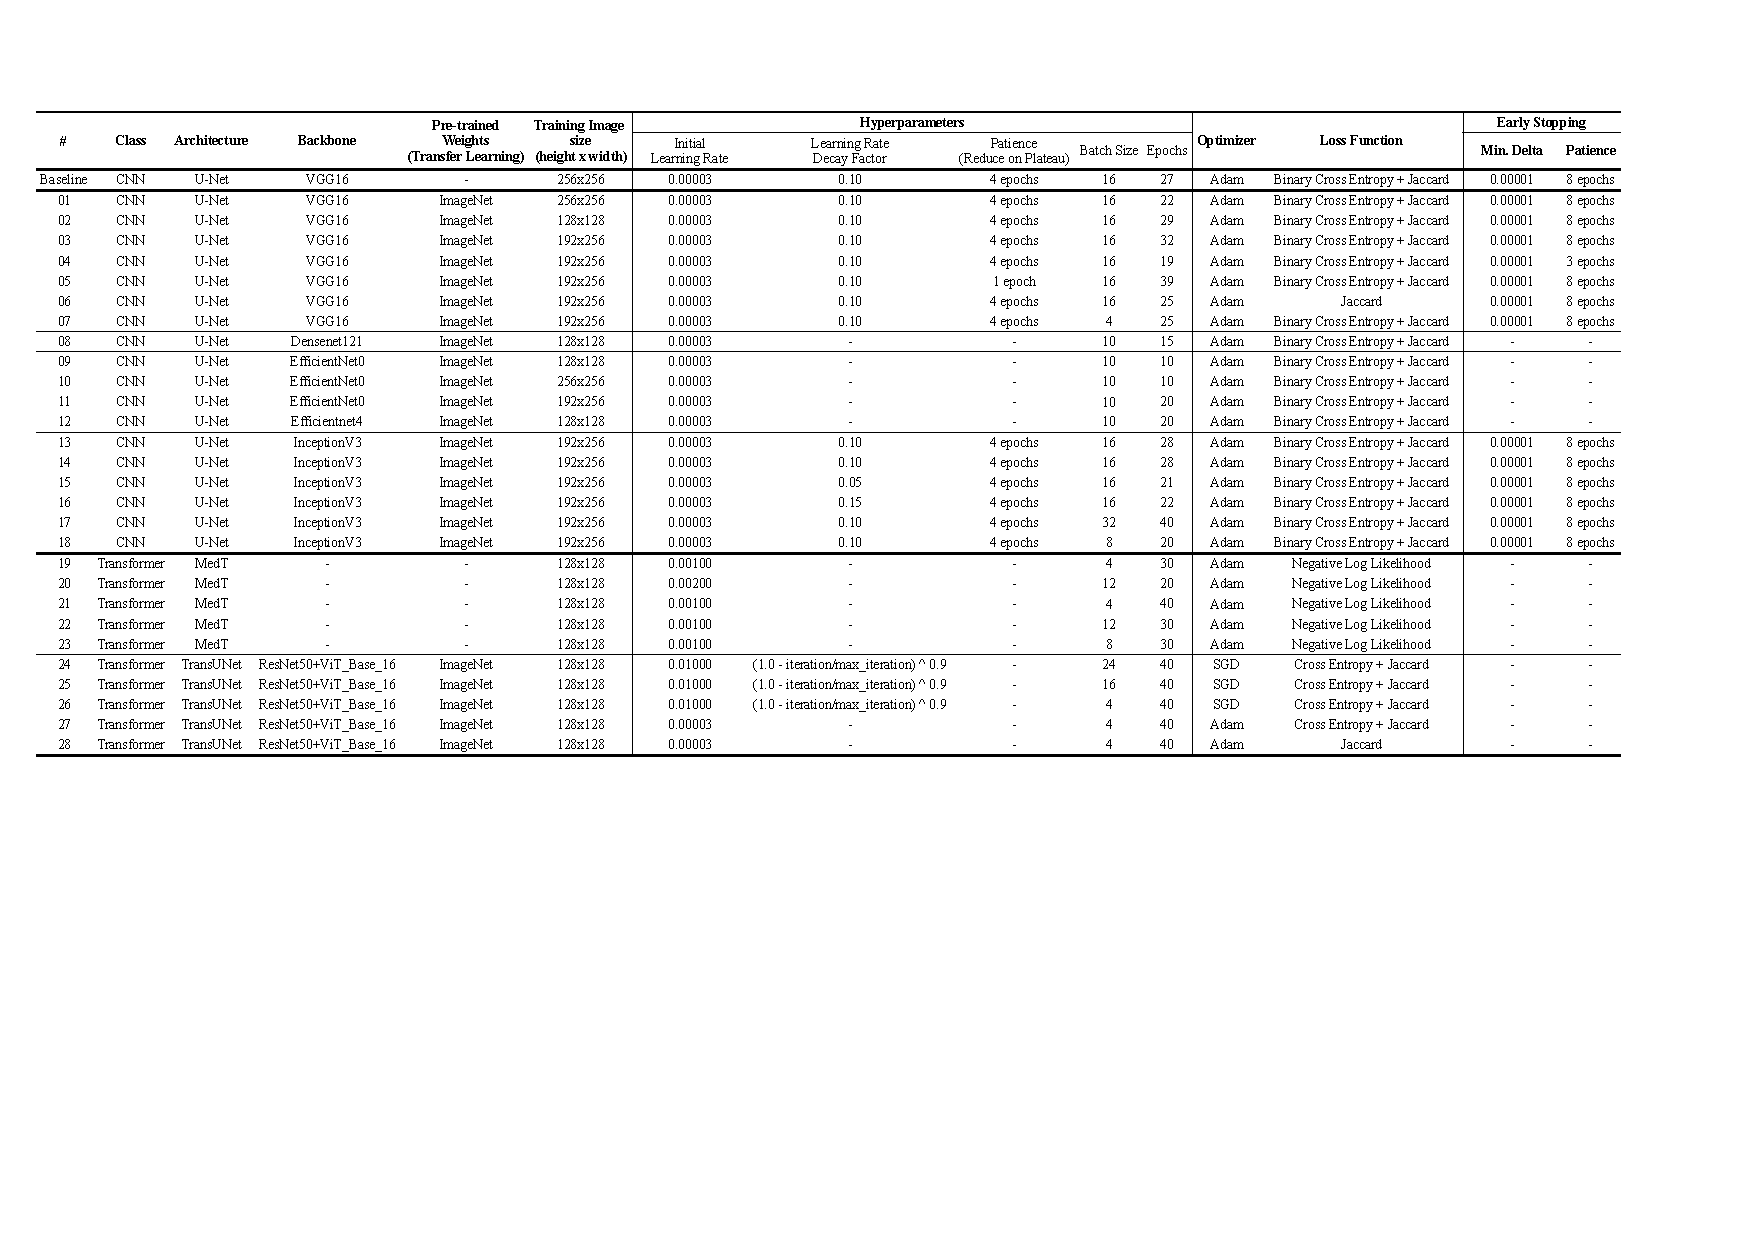
\includegraphics[width=\textwidth]{assets/experiments.pdf}
  \caption[Experiments]{Experimental model configurations with hyperparameter settings, optimizer, loss function and early stopping setup. First row corresponds to the baseline model.}
  \label{table:experiments}
\end{table*}

We used the following three machine learning frameworks as our experiment design guide:

\textbf{Ablative Analysis}: In order to determine the optimal image size for each model given the time and resources constraints, we performed ablation studies with input resolutions of 512x512 pixels, 2556x256 pixels, 192x256 pixels and 128x128 pixels. We also study the impact of transfer learning on the selected model architecture by adding or removing encoder weights pretrained on ImageNet. Furthermore, we study the effect of different encoder backbones in our encoder-decoder architectures.

\textbf{Approximation and estimation error}: We use the accuracy metrics to measure the performance of the models during training and inference time. We test different data preprocessing techniques like removing or adding hair to measure how much error is attributable to each method.

\textbf{Bias-variance diagnostic}: We use various regularization techniques like early stopping to understand the bias-variance trade-off and to prevent the models from overfitting in order to generalize well on unseen data. For final performance comparison, we report all previously defined metrics on an unseen test dataset.


\subsection{Conclusion}

Table \ref{table:results} summarizes all experiment results. The models were trained with different image input sizes, harmonized and downscaled from the original images resolutions. The final averaged evaluation metrics were calculated on unseen test dataset. The predicted image masks were upscaled to the original image resolution from the test dataset and compared with its corresponding binary mask. We report six different metrics: Threshold Jaccard Index, Jaccard Similarity Index, Dice Coefficient, Accuracy, Sensitivity and Specificity.

\begin{table*}[ht]
  \centering
  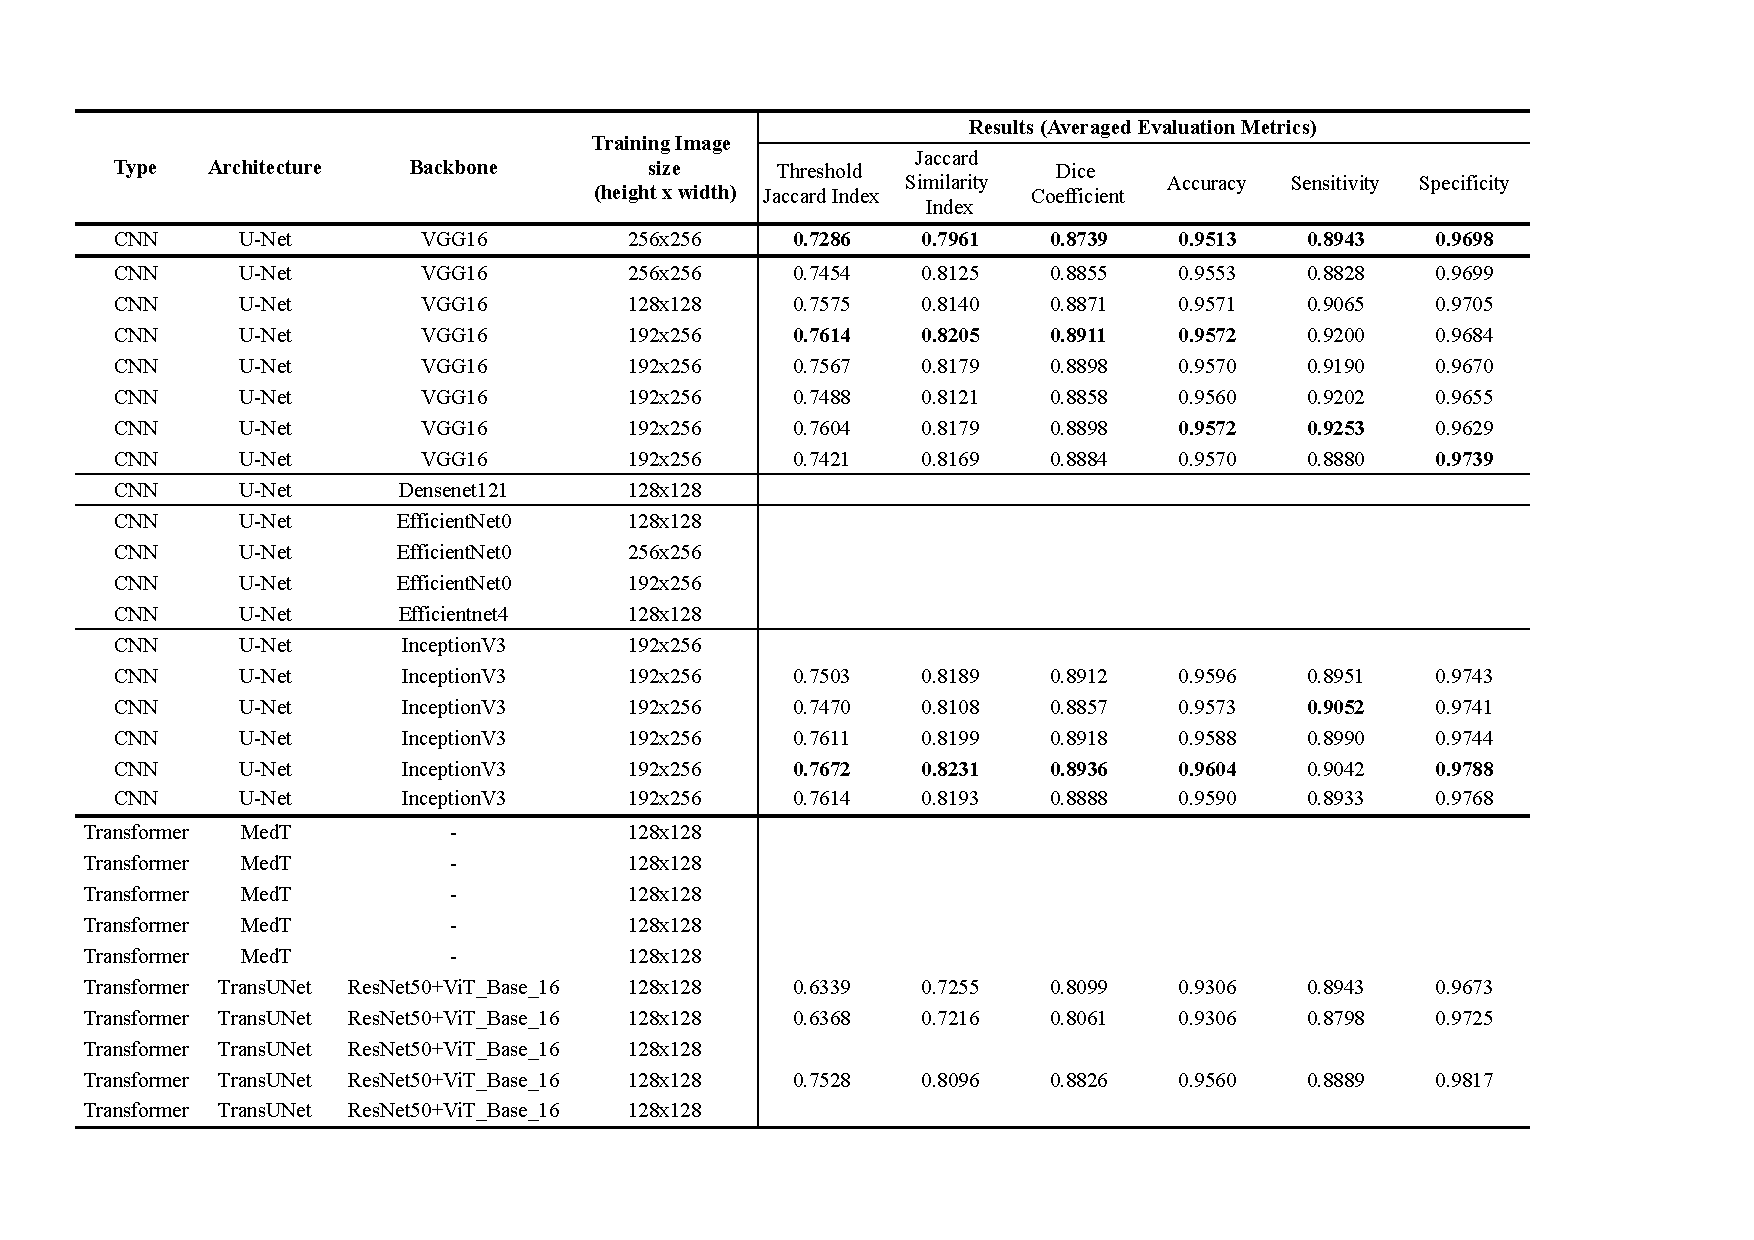
\includegraphics[width=\textwidth]{assets/results.pdf}
  \caption[Results]{Model flavors with corresponding type, architecture, input image sizes and final results as reported on unseen test dataset. First row corresponds to the baseline model.}
  \label{table:results}
\end{table*}

The first row shows the results of the baseline U-Net model configuration using the VGG16 backbone with no pre-trained weights, followed by the CNN models with different backbone  flavors. The last section presents the results of Transformer based models, namely MedT and TransUNet. Best performing models setups and their metrics are highlighted in bold.

\par
Our best performing CNN-based model was able to outperform the baseline model by 3.86\% on the Threshold Jaccard Index. Our best performing transformer configuration, TransUNet with pre-trained weights on ImageNet and ResNet50+ViT\_Base\_16 as backbone, was able to outperform the baseline model by 2.46\% as measured by the same metric.

\par
While we weren’t able to show that Transformers outperform CNN based models as measured by the Threshold Jaccard Index, we show that the performance is still very much comparable. Looking at other metrics, the Dice Coefficient difference is only 1.03\%, accuracy about 0.47\% while sensitivity is slightly higher with 2.1\% divergence. However, TransUNet shows a 0.32\% improvement over the best performing InceptionV3 backbone. This improvement comes with much higher computational cost compared to CNN based networks though (around double the training time).

\par
CNN based models were trained on different image sizes (ablation study) as they are image size agnostic. We show that preserving the image aspect ratio of the original image seems to boost the overall model performance on the metrics. Transformer based models were trained with a fixed size of 128x128 pixel using 16x16 image patches, following the recommendation of the authors \citep{transunet-2021-chen, medical_transformer-2021-valanarasu}. In general, a bigger image resolution while training seems to preserve the segmentation details better and hence leads to better performance. This observation goes in hand with the ablation studies performed by \citep{transunet-2021-chen}.

\par
Image preprocessing as well as data augmentation plays a crucial role for image segmentation, especially when the input images show different characteristics in terms of quality as well as data scarcity. In our experiments we observed that adding noise to the image like e.g. artificial hair or random gaussian noise performs better than removing noise (e.g. removing hairs) from the images as proposed by \citep{data_purification-2019-bisla} and shown in experiment 13. This seems counterintuitive at first. A possible explanation would be that the added noise helps to even out the underrepresentation of occluded images and hence makes the networks more robust \citep{skin_segmentation-2019-jahanifar} come to the same conclusion. We also experimented with the seam carving technique \citep{seam_carving-2007-shai} in order to preserve as much of the valuable and important information while compressing images. The results of this preprocessing method did not meet our expectations and were not pursued further.

\par
We used the Adam optimizer in most of our experiments as it showed the best performance as compared e.g. to SGD. We observed in some cases that using only the Jaccard loss function may lead to performance boost compared to combination of binary cross entropy with Jaccard loss. During hyperparameter tuning our experiments show that decreasing the batch size from 16 to 4 leads to a better outcome for the Transformer architecture. CNN based architectures show the opposite behaviour. We also show that using pre-trained weights on ImageNet (Transfer Learning) for the encoder part helps to boost the models performance both for CNN based as well as Transformer based models and significantly shortens the training time.


% \begin{itemize}
%   \item Describe all Machine Learning Theory techniques used to evaluate the success of the model.
%   \item Describe how results compare to previous research.
% \end{itemize}
